\documentclass{article}
\usepackage[utf8]{inputenc}
\usepackage[T1]{fontenc}
\usepackage[francais]{babel}
\usepackage{hyperref}
\usepackage{parselines}
\hypersetup{
unicode=false, % non-Latin characters bookmarks
pdftoolbar=false, % show Acrobat's toolbar?
pdfmenubar=false, % show Acrobat's menu?
pdffitwindow=true, % page fit to window when opened
pdftitle={Rapport Genie logiciel}, % title
pdfauthor={REYNAUD Nicolas}, % author
pdfsubject={thèse}, % subject of the document
pdfnewwindow=true, % links in new window
colorlinks=true, % false: boxed links; true: colored links
linkcolor=black, % color of internal links
citecolor=green, % color of links to bibliography
filecolor=magenta, % color of file links
urlcolor=blue % color of external links
}
\usepackage{manyfoot}
\usepackage[stable]{footmisc}
\usepackage{geometry}
\usepackage{graphicx}
\usepackage{amssymb}
\geometry{hmargin=3.0cm,vmargin=1.5cm}
\title{Rapport Reunion \#4}
\author{Kevin \bsc{Bascol}}
\date{29 Octobre 2014}
\begin{document}
\maketitle
\newpage

Réunion effectuée en ligne via Skype.\\
Présents à la réunion: Kévin Laoussing, Nicolas Reynaud et Kevin Bascol.

\subsection*{Ordre du jour}
	\begin{itemize}
		\item Interface graphique.
		\item Structure du document de spécification des exigences.
	\end{itemize}

\subsection*{Bilan du travail}
	\begin{itemize}
		\item Chaque membre est à jour dans l'écriture des exigences comme décidé à la réunion précédente.
		\item Le planning a été mis à jour et en ligne.
	\end{itemize}
	
\subsection*{Décisions de la réunion}
	\begin{itemize}
		\item Nous avons dessiné l'esquisse de l'interface graphique.
		\item Nous avons réparti les exigences de l'interface graphique. Chaque personne écrira les exigences correspondant aux fonctionnalités dont il était responsable, en accord avec l'esquisse.
		\item Nous avons sélectionné les sous parties que nous allons conserver du modèle de document de spécification des exigences qu'on avait choisit précédemment.
	\end{itemize}
	
\subsection*{Prévision du travail}
	\begin{itemize}
		\item Chaque membre devra écrire les exigences dont il est responsable.
		\item Kevin Bascol devra mettre en commun le travail de chacun.
	\end{itemize}
	
\subsection*{Prochaine réunion: 4 novembre 2014}
	\textbf{Ordre du jour:} préparation du cahier de conception générale.
	
\subsection*{Remarque}
\begin{itemize}
\item Utilisation d'un site de dessin collaboratif dans le but de réfléchir l'interface graphique ensemble. http://flockdraw.com/.
\item Pour des raisons de disponibilité des membres la réunion a été reportée du 28 octobre au 29 octobre.
\end{itemize}

\newpage

\subsection*{Annexes}
Esquisses des interfaces\\
\begin{center}
	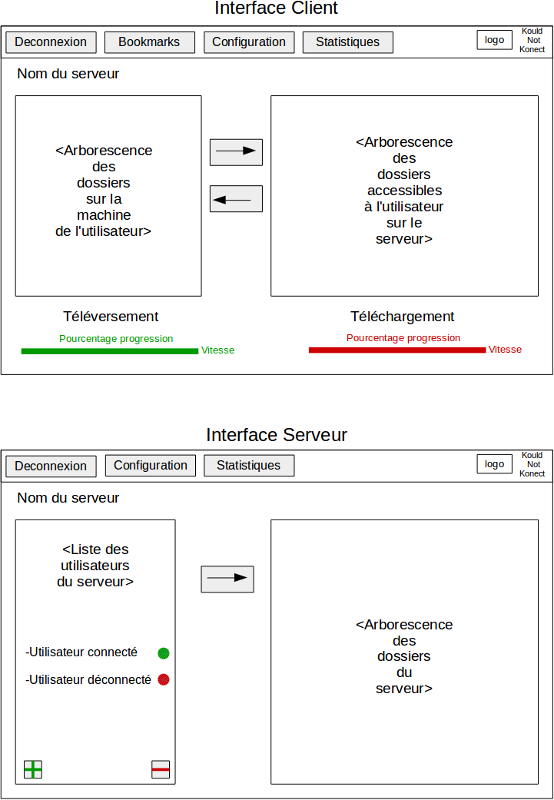
\includegraphics{Interface_projet_gl.png}
\end{center}

\end{document}
